\documentclass[conference]{IEEEtran}
\usepackage[utf8]{inputenc}
\usepackage{amsmath,amssymb,amsfonts}
\usepackage{graphicx}
\usepackage{cite}
\usepackage{hyperref}
\usepackage{url}
\usepackage{balance}

\title{Mobile Application for Crowdsourced GNSS Spoofing Detection}

\author{
 \IEEEauthorblockN{Nathan Johnson}
 \IEEEauthorblockA{
    Cyber Intelligence and Security Department\\
    Embry-Riddle Aeronautical University\\
    Prescott, Arizona, USA\\
    johnsn63@my.erau.edu
  }
}

\begin{document}

\maketitle

\begin{abstract}
Global Navigation Satellite Systems (GNSS) play a critical role in modern infrastructure, from aviation and maritime navigation to time synchronization for cryptographic systems. However, the increasing reliance on GNSS has made it a valuable target for cyber threat actors, particularly through GNSS spoofing attacks. Unlike jamming, which simply disrupts GNSS signals, spoofing can deceive systems into using false positional data, leading to potentially severe consequences. This paper explores a novel approach to GNSS spoofing detection using mobile devices, leveraging onboard GNSS receivers and inertial sensors. Initial findings reveal significant limitations in consumer-grade accelerometers and gyroscopes for implementing a full Inertial Navigation System (INS). However, a simpler detection method based on monitoring deviations in GNSS position over time was developed. While this approach shows promise, false positive detections due to inherent GPS inaccuracies remain a challenge. Future work will focus on refining detection methods, potentially incorporating machine learning and noise reduction techniques to improve reliability.
\end{abstract}

\begin{IEEEkeywords}
GNSS, GPS spoofing, mobile security, inertial navigation system, cybersecurity, Android, sensor fusion, machine learning
\end{IEEEkeywords}

\section{Introduction}
Global Navigation Satellite Systems (GNSS) are satellite-based systems that provide geolocation and time information to a GNSS receiver anywhere on or near the Earth. Major systems include the American GPS, Russian GLONASS, EU Galileo, and Chinese BeiDou. These systems rely on atomic clocks in space and one-way communication to deliver precise timing and positional data.

GNSS is a cornerstone of modern infrastructure. It is used in military operations, aviation and marine navigation, civilian navigation systems, autonomous vehicles like self-driving cars and drones, and global time synchronization for systems like the internet and cryptographic protocols\cite{lu2021}. As such, the loss or manipulation of GNSS signals could have serious implications.

GNSS systems fall under the broader category Position Navigation and Timing (PNT) systems. GPS-based navigation in aviation, for instance, is quickly replacing ground-based navigation methods due to its flexibility and lower costs\cite{meng2021}.

\section{Threats}
GNSS jamming is a basic denial of service (DoS) technique. It involves overpowering the weak satellite signals with noise transmitted at known GNSS frequencies. This disrupts service but is easy to detect due to the total loss of signal.

GNSS spoofing, however, is far more insidious. It undermines data integrity by impersonating legitimate satellites. Spoofed signals are carefully crafted to look valid and can gradually diverge from true signals, making detection difficult. Spoofing is well within the capabilities of nation-state actors and can be executed with increasing sophistication, such as by gradually increasing deviation to avoid triggering alarms.

Spoofing poses a major risk to sectors that depend on GPS integrity. For example, spoofing can misdirect military drones, compromise aviation safety, or impact time-synchronized cryptographic systems. Known spoofing hotspots include regions of geopolitical conflict, where such attacks have been regularly reported.

\section{Detection Methods Overview}
There are several different approaches that have been used to detect GNSS spoofing.

Comparison to known good positions is a very simple method and involves comparing the current GNSS-derived position with a trusted reference location. If significant deviation occurs especially in a stationary device it may indicate spoofing. This approach is useful in fixed-location infrastructure or crowd-sourced detection networks.

Satellite and ground-based augmentation systems (SBAS, GBAS) provide correction data and integrity information to receivers. Spoofing attempts that contradict augmentation data can be flagged. These systems enhance both positional accuracy and spoofing detection.

Inertial Navigation System (INS) comparison relies on gyroscopes and accelerometers to estimate movement. Spoofing detection compares the inertial-based path to the GNSS path. Divergence between these two sources, particularly in the short term, may suggest spoofing.

These strategies can be combined into hybrid approaches for greater performance.

\section{Signal Strength Based Spoofing Detection}
One method of detecting spoofing attacks involves monitoring the signal strength of received GNSS signals. Due to the satellites’ far distance from Earth, legitimate GPS signals are extremely weak by the time they reach the surface. This received power level is also highly consistent over large geographical areas\cite{lo2021}.

In contrast, spoofed GPS signals originate from transmitters much closer to the receiver. Because of this proximity, the received signal strength can vary significantly based on the distance from the spoofing source. Spoofing attacks rely on overpowering the legitimate satellite signals to deceive the receiver. As a result, spoofed signals are often substantially stronger than authentic signals. Monitoring for unexpected increases in signal strength can therefore be used as an indicator of a potential spoofing attack\cite{lo2021}.

A method used in Google's GNSS Logger evaluates the Carrier-to-Noise ratio (C/N0) and Automatic Gain Control (AGC). An increase in C/N0 alongside a decrease in AGC typically signals a stronger than expected GNSS signal and may indicate spoofing\cite{spens2022}. This will be implemented in the current version of the detection app.

\section{Methodology}
The prototype was developed using Android Studio in Java. A Google Pixel 7 Pro was used for testing, leveraging its onboard GNSS, accelerometers, and gyroscopes. The initial approach aimed to implement a basic Inertial Navigation System (INS), comparing calculated motion from integrated sensor data to GPS data.

SpoofDetect V1 attempted to perform double numerical integration of acceleration to derive velocity and position, but consumer-grade accelerometers proved wildly inaccurate (±1 m/s²). Additionally, raw GPS data showed variations of ±10 meters.

\begin{figure}[htbp]
    \centerline{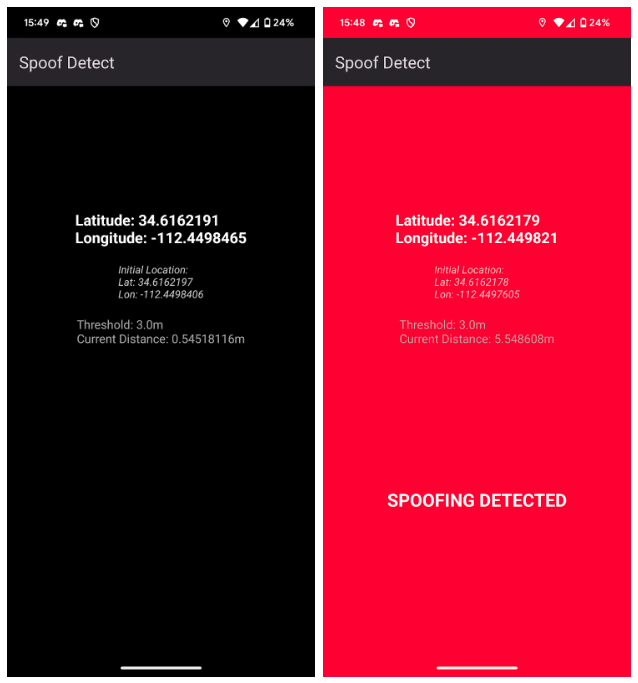
\includegraphics[width=0.5\textwidth]{figs/spoofdetect_app.png}}
    \caption{Screenshot of SpoofDetectV1 Android app.}
   \end{figure}

SpoofDetect V2 implemented Google’s C/N0 and AGC-based method. The app processes the last 10 and 60 epochs of data to detect anomalies in signal strength patterns. The app appears to be working almost perfectly. Testing with synthetic data yielded promising results, showing few false positives and no observed false negatives.

\begin{figure}[htbp]
    \centerline{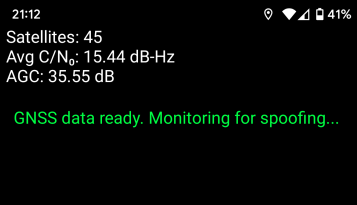
\includegraphics[width=0.5\textwidth]{figs/spoofdetectv2.png}}
    \caption{Screenshot of SpoofDetectV2 Android app.}
   \end{figure}

\section{Next Steps}
A future goal for this project is to create a global, real-time GNSS spoofing detection network. The vision is to have the SpoofDetect app report detections back to a centralized server. This server would aggregate detection reports from mobile devices worldwide, enabling the system to map spoofing events as they occur.

By crowdsourcing detection data from consumer devices, the network could monitor spoofing activity in real time and identify trends or hotspots. Critical GNSS users such as aircraft, autonomous vehicles, maritime vessels, or infrastructure systems could then receive alerts or advisories when spoofing activity is detected in their area. This would help mitigate risk, improve situational awareness, and increase resilience against GNSS-based threats.

Eventually, the centralized detection server could also integrate external augmentation systems and validation services, such as SBAS or Doppler-based verification, to further strengthen spoofing detection and classification.


\section{Conclusion}
The investigation into GNSS spoofing detection using mobile devices has demonstrated both the potential and limitations of consumer-grade hardware for this application. While inertial-based methods suffer from sensor inaccuracies, signal strength monitoring and augmentation with techniques like machine learning and aggregation show significant promise. As GNSS spoofing continues to grow as a cybersecurity threat, developing accessible and effective detection methods remains an important pursuit.

The source code for this project is available on github.
https://github.com/nJohnson02/gps-spoofing-detection

\bibliographystyle{IEEEtran}
\bibliography{references}
\nocite{*}
\balance{}

\end{document}
